\documentclass[fleqn, a4paper. 12pt]{ltjsarticle} % lualatex guidance.tex
\usepackage{amsmath,txfonts}
\usepackage{amssymb}
\usepackage{url}
\usepackage[margin=31mm]{geometry}
\usepackage{graphicx}
\usepackage{color}

\newcommand{\XA}[1]{\begingroup \color{red}}
\newcommand{\AX}[1]{\endgroup}

\newcommand{\br}[1]{\left(#1\right)}                %normal brackets
\newcommand{\cbr}[1]{\left\{#1\right\}}             %curly brackets
\newcommand{\sbr}[1]{\left\lbrack #1 \right\rbrack} %square brackets

\usepackage{listings} 

\lstset{
  basicstyle={\linespread{0.6}},
  identifierstyle={\small},
  keywordstyle={\small\bfseries},
  ndkeywordstyle={\small},
  stringstyle={\small\ttfamily},
  frame={tb},
  breaklines=true,
  columns=[l]{fullflexible},
%  numbers=left,
  xrightmargin=1em,
  xleftmargin=2em,
  numberstyle={\scriptsize},
  stepnumber=1,
  numbersep=1em
}

\begin{document}
    \begin{titlepage}
      \begin{center}
      {
      \Huge 2023年度\\システムプログラミング実験}
      
      \vspace{4cm}
             {\Huge 第2回\\テクニカルライティング\\
               実験レポート\\}
             \vspace{4cm}
                    {\large 実験日:2023年10月10日(水)\\提出日:2023年10月10日(水)\\}
                    
                    {\large 学修番号:22140003\\氏名:佐倉仙汰郎}
    \end{center}  
  \end{titlepage}
  \newcommand{\fB}{f_\mathrm{B}}
  \newcommand{\fQ}{f_\mathrm{Q}}
  \newcommand{\fM}{f_\mathrm{M}}
  \newcommand{\fSTL}{f_\mathrm{STL}}

    \section{初めに}
    本書ではシステムプログラミング実験第2回の課題を実施した結果を報告する.課題は4つの異なるソートの手段について、計算量の違いについて解析するものである.解析結果をグラフに示し、その結果について考察を行う.
    \section{実験の説明}
    整列アルゴリズムの計算時間を計測し,その結果に基づき性能を評価する.
    評価を行うアルゴリズムは、
    \begin{itemize}
        \item バブルソート: $\fB$
        \item クイックソート: $\fQ$
        \item マージソート: $\fM$
        \item C++ Standard Template Library\footnote{\url{https://www.boost.org/sgi/stl/doc_introduction.html}} のsort関数によるソート: $\fSTL$
    \end{itemize}
    の4つである.
    これらの整列ソートは要素数を$N$として,$\fB(N) = O(N^2), \fQ(N) = O(N\ln N), \fM(N) = O(N\ln N)$となる。計算量の違いがどのように計算時間に影響するかを図を用いて解析していく.
    上記ソートについて計測を行い,横軸を要素数,縦軸を実行時間としたグラフを作成する.そして横軸縦軸は対数軸を使用する.
    要素数$N$については対数軸をとるため、第$k$回の実験における要素数を$N_k$とし、次の式(1)に示す.
    \begin{equation}
      \label{e3}
      M_k = 1.2M_{k-1}, N_k = R(M_k), k=1,2,...,K-1.
    \end{equation}
    ここでは$M_1 = 32$を選択した.$M_1$の値が小さすぎると処理回数が増えるだけで、計算量の差異がわかりやすくなるわけではない.
    計算量の違いは$N$の値が大きくなる時に差が出るので$M_1 = 32$は妥当な値である.
    今回は前述したとおり対数軸を使うので、$N$の値は等比数列で設定した.
    このようにして生成したデータ点の 2 次元グラフによる可視化と,実際の数値の値から結果を考察
    する.
  \section{実験結果}
  前節で説明した方法をC++言語により実装した.実装環境は以下のとおりである.
  \begin{itemize}
    \item Central Processing Unit: 11th Gen Intel(R) Core(TM) i7-1167G7 @ 2.80 GHz
    \item 主記憶: Double Data Rate 4 Synchronous Dynamic Random-Access Memory
    \item コンパイラ: g++ version 11.2.0
    \item コンパイルコマンド: g++ -std=c++14 sort.cpp (sort.cpp はソースプログラムのファイル名である.)
    \item Operating System: Arch Linux\footnote{\url{https://archlinux.org/}}
    \item 数値型: 倍精度浮動小数点数\footnote{\url{https://www.gnu.org/software/gsl/doc/html/ieee754.html}}
  \end{itemize}
  \begin{figure}[tb]
    \label{f1}
    \centering
    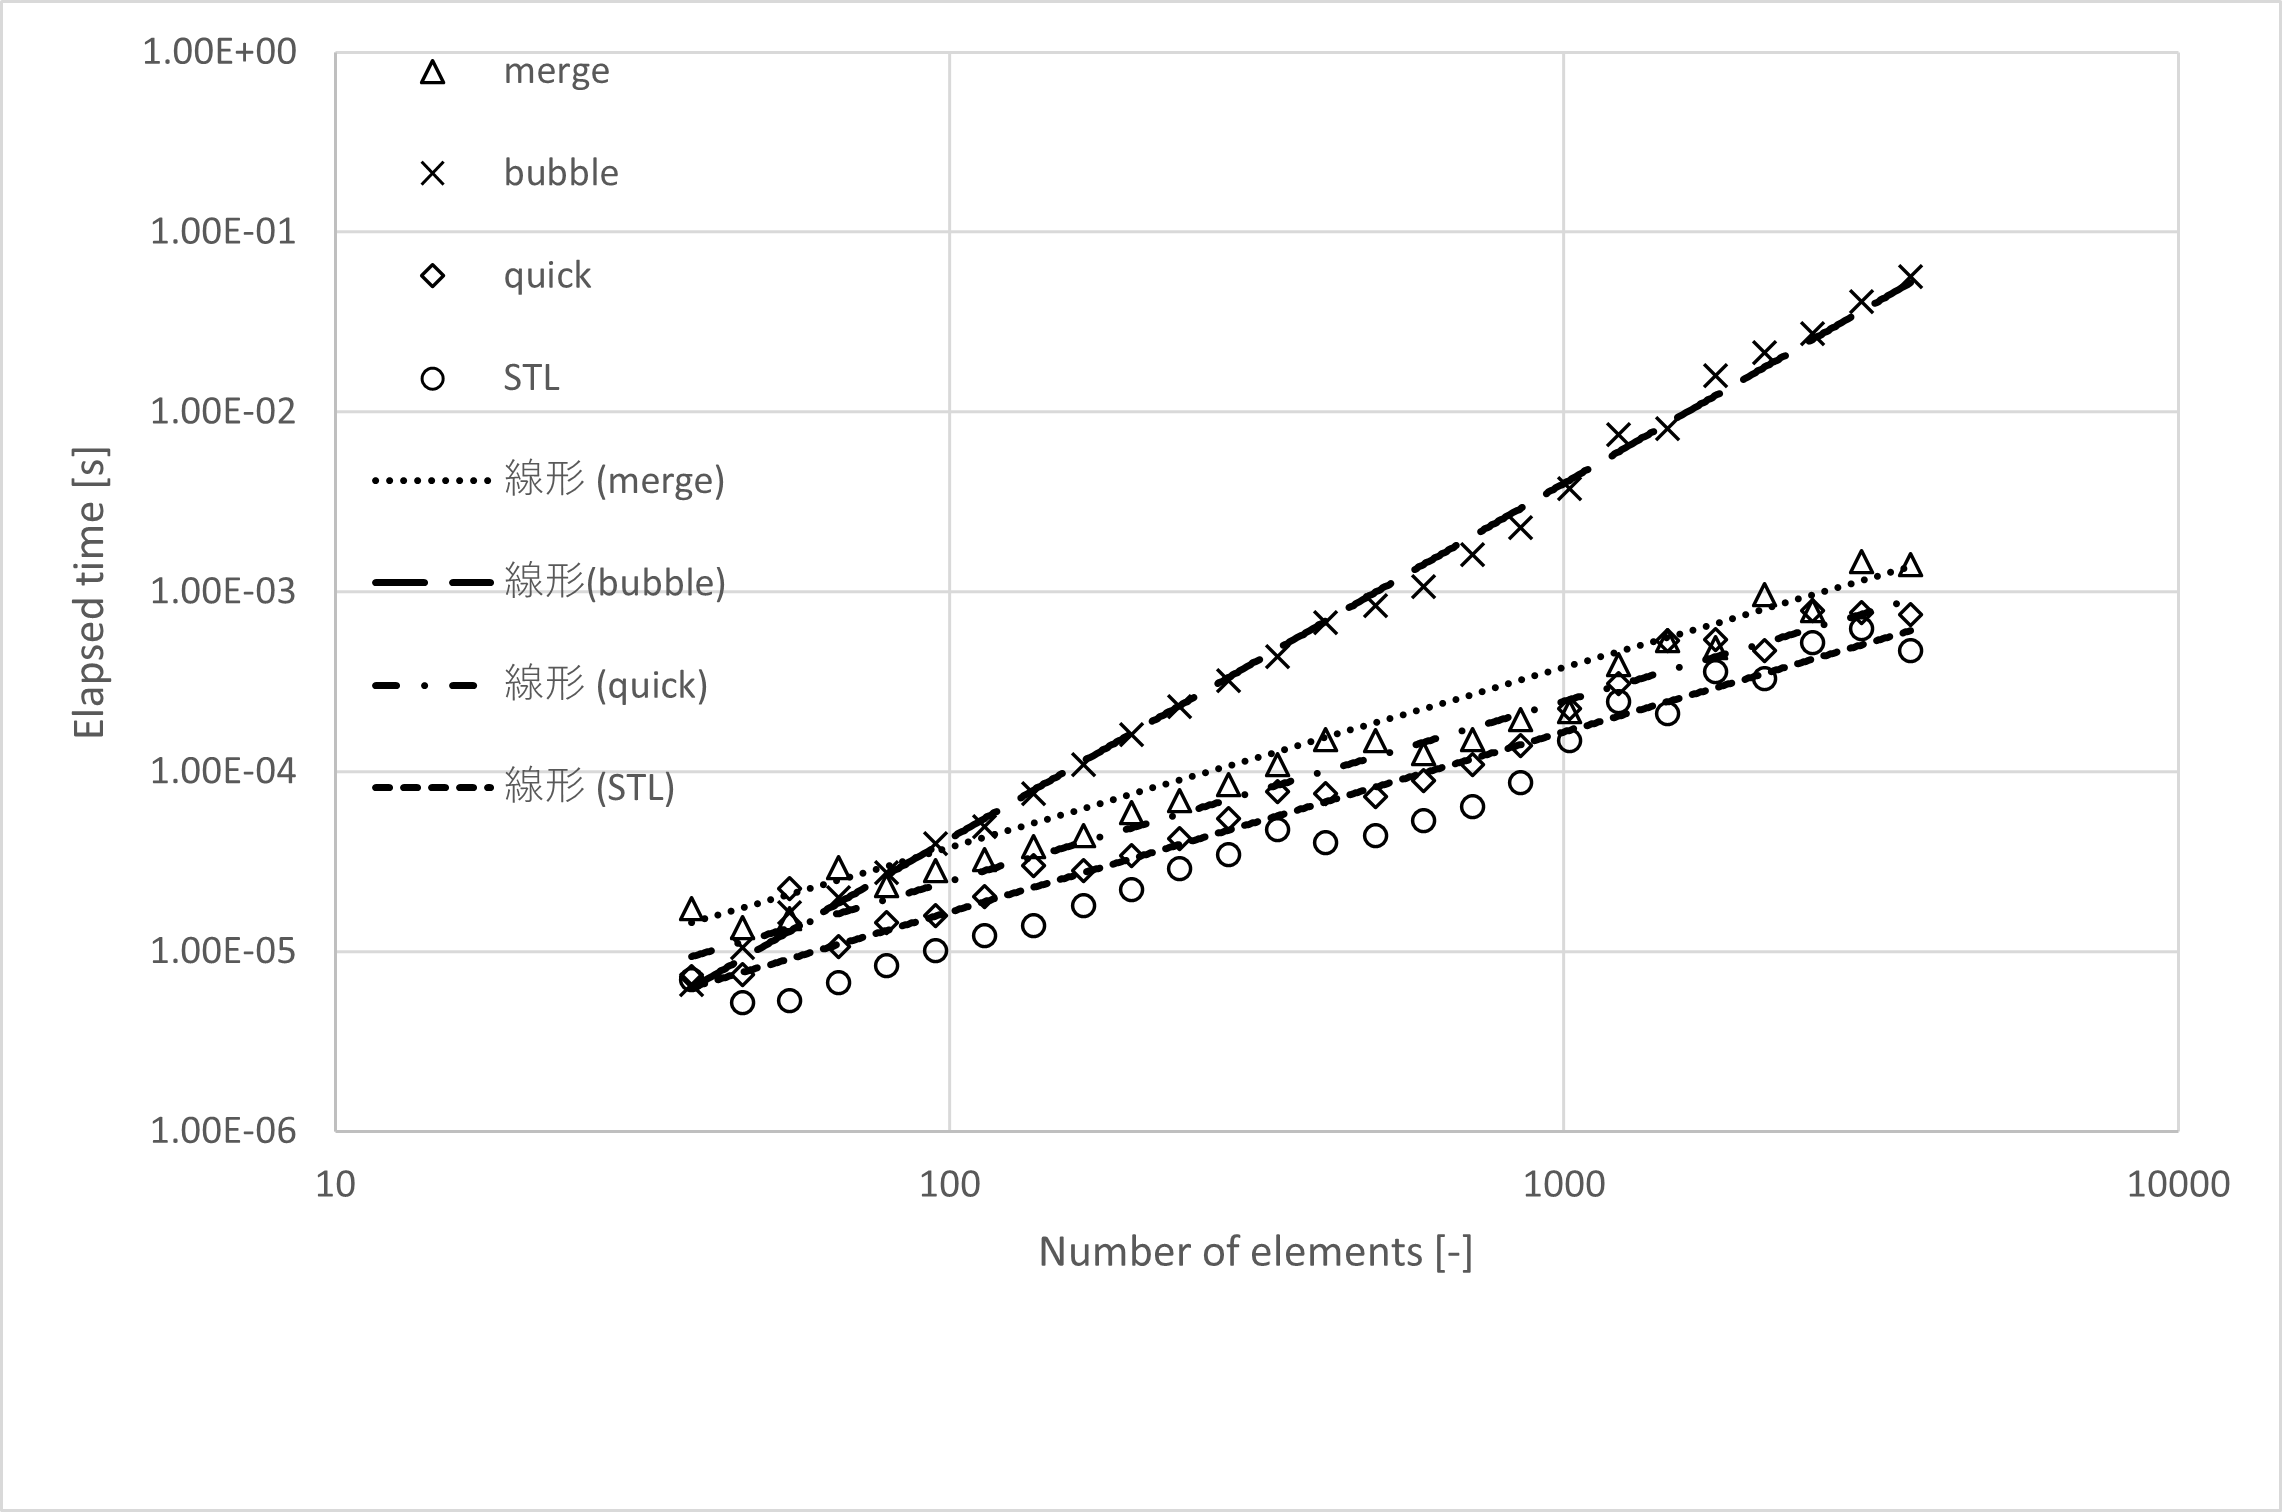
\includegraphics[width=\textwidth]{zu2.png}
    \caption{実験結果のグラフ.4つのソートアルゴリズムの計算時間が縦軸、横軸が試行回数$N$になっている.}
  \end{figure}
  4つの異なるソートアルゴリズムの計算量とそれに用いた要素数を軸とした図を示す.
  この図からバブルソートの計算量が$N$の値が大きくなるとほかのアルゴリズムの計算量との差が大きくなることが分かる.
  ほか3つのアルゴリズム、クイックソート、マージソート、C++ Standard Template Libraryに関しては回帰直線の傾きがある程度近似していることが分かる.
  バブルソートの計算量が$O(n^2)$であることから、図(1)のバブルソートの回帰直線の傾きはおおよそ2になっている。
  ただし、これらの3つのソートアルゴリズムに有意な差はこの図からは読み取れないため、実際の数値を読み取る必要がある.\\
  表(1)より、$N<=66$の範囲では、バブルソートはマージソートよりも計算時間がかかっている.
  STLのソートは$N$のすべての範囲で計算量が一番早い.クイックソートはSTLのソートの次に早いことがこの表(1)からわかった.
  \begin{table}[tb]
    \caption{要素数$N$に対する4つのアルゴリズムの計算時間である.}
    \begin{tabular}{lllll|lllll}
    \hline
    N   & merge     & bubble    & quick     & STL       & N    & merge     & bubble    & quick     & STL       \\ \hline
    38  & 0.0000173 & 0.0000065 & 0.0000073 & 0.0000070 & 410  & 0.0001500 & 0.0006722 & 0.0000756 & 0.0000404 \\
    46  & 0.0000136 & 0.0000105 & 0.0000074 & 0.0000052 & 493  & 0.0001495 & 0.0008352 & 0.0000727 & 0.0000443 \\
    55  & 0.0000152 & 0.0000165 & 0.0000223 & 0.0000054 & 591  & 0.0001252 & 0.0010661 & 0.0000891 & 0.0000533 \\
    66  & 0.0000291 & 0.0000198 & 0.0000107 & 0.0000067 & 709  & 0.0001498 & 0.0016033 & 0.0001094 & 0.0000639 \\
    79  & 0.0000232 & 0.0000275 & 0.0000144 & 0.0000084 & 851  & 0.0001954 & 0.0022816 & 0.0001388 & 0.0000863 \\
    95  & 0.0000283 & 0.0000400 & 0.0000158 & 0.0000101 & 1022 & 0.0002156 & 0.0037578 & 0.0002237 & 0.0001496 \\
    114 & 0.0000324 & 0.0000494 & 0.0000203 & 0.0000123 & 1226 & 0.0003923 & 0.0074607 & 0.0003071 & 0.0002443 \\
    137 & 0.0000384 & 0.0000750 & 0.0000299 & 0.0000139 & 1472 & 0.0005330 & 0.0080440 & 0.0005325 & 0.0002096 \\
    165 & 0.0000438 & 0.0001100 & 0.0000282 & 0.0000179 & 1766 & 0.0004890 & 0.0158310 & 0.0005427 & 0.0003573 \\
    198 & 0.0000592 & 0.0001612 & 0.0000339 & 0.0000221 & 2119 & 0.0009590 & 0.0212213 & 0.0004713 & 0.0003282 \\
    237 & 0.0000692 & 0.0002304 & 0.0000426 & 0.0000290 & 2543 & 0.0007882 & 0.0273119 & 0.0007873 & 0.0005225 \\
    285 & 0.0000850 & 0.0003221 & 0.0000549 & 0.0000346 & 3052 & 0.0014629 & 0.0411523 & 0.0007628 & 0.0006274 \\
    342 & 0.0001092 & 0.0004362 & 0.0000769 & 0.0000477 & 3663 & 0.0014079 & 0.0568365 & 0.0007464 & 0.0004689 \\ \hline
    \end{tabular}
    \label{t1}
    \end{table}

  \section{考察}
  今回の実験により計算量の違いが有意な差であることがわかった.$O(n^2)$であるバブルソートは図(1)からわかるように計算時間が寄りかかった.
  このことからバブルソートは膨大なデータに向かないこず、ほかのソートアルゴリズムを検討することが妥当である.
  また今回の実験で、計算量が同じソートアルゴリズムでも、それぞれに特徴があることが分かった.
  マージソートは計算量が$O(nlogn)$でクイックソートと等しいが、$N$の値が小さいときにはクイックソートよりも遅いので、使い場合を選ぶ.
  以上より、アルゴリズムを選択するときには使用するデータセットの特徴を見極めそれに適したものを選ぶ必要があることがわかった.
  今回使用したソートアルゴリズムの中で唯一具体的な計算量が分からないSTLのソートだが、クイックソートとマージソートと大差ないことから、$O(nlog(n))$であると考えるのが妥当だろう.

  \section{おわりに}
    本書ではシステムプログラミング実験の課題として、整列アルゴリズムの計算時間を計測し,その結果に基づき性能を評価した。結果として計算量の違いにより計算時間に大きな差が出ることがわかった。また同じ計算量のアルゴリズムでもそれぞれに特色があり、状況に応じてソートアルゴリズムを選択する必要があることがわかった.
    \section{付録}
    図(1)の作成に用いたソースコードをここに記載する。
    \begin{figure}[b]
      \begin{lstlisting}[mathescape=true, numbers=left]
        #include <iostream>
        #include <random>
        #include <string>
        #include <chrono>
        #include <functional> // function library to define a function in a function
        #include <fstream>
        #include <algorithm>
        
        using namespace std;
        
        void mergeSort(int* vA, int N)
        {
            int* vM = vA;
            int* vMt = new int[N];
            function<void(int, int, int)> merge = [&](int left, int mid, int right) { // lambda function.
            // このラムダ関数を使えば,再帰関数を定義するのに,わざわざグローバル領域に関数を宣言せずにすむ.
            // ラムダ関数は関数の中に宣言できる特別な関数である.
            // 宣言された関数内のローカル変数を参照できる.
            // 構文は,14行目のとおりである.
            // - function: ラムダ関数を入れる特別なクラス
            // - void(int, int, int): 関数の型.int の引数がmergeソートの要件から3つほしいため,このように定義している.返り値必要ないため void とした.
            // = [&](int left, int mid, int right){}: 関数の処理内容の定義.& はローカル変数をラムダ関数の中で改変可能とする宣言.ほかは普通の関数と同様の意味
                int il = 0;
                int ir = 0;
                int el = mid - left;
                int er = right - mid;
                while (true) {
                    if (il == el) {
                        if (ir == er) {
                            return;
                        } else {
                            vMt[left + il + ir] = vM[mid + ir];
                            ++ir;
                        }
                    } else {
                        if (ir == er) {
                            vMt[left + il + ir] = vM[left + il];
                            ++il;
                        } else {
                            auto tl = vM[left + il];
                            auto tr = vM[mid + ir];
                            if (tl <= tr) {
                                vMt[left + il + ir] = tl;
                                ++il;
                            } else {
                                vMt[left + il + ir] = tr;
                                ++ir;
                            }
                        }
                    }
                }
            };
            function<void(int, int)> mergeSort = [&](int left, int right) {
                //ラムダ関数は関数内で複数定義可能.
                if (right - left <= 1) {
                    return;
                }
                auto mid = (left + right) / 2;
                mergeSort(left, mid); // 普通の関数と同じように,ラムダ関数を呼び出し可能.ただし,宣言された関数(スコープ)外からラムダ関数を呼び出すことはできない.この性質はローカル変数と同じものである.ラムダ関数の枠組みでは関数を変数のように扱うことが可能となっている.
                mergeSort(mid, right);
                merge(left, mid, right);
                for (int i = left; i < right; ++i) {
                    vM[i] = vMt[i];
                }
            };
            mergeSort(0, N);
            delete [] vMt;
        }
        void quickSort(int* vA, int N)
        {
        
            function<void(int, int)> sort = [&](int is, int ie) {
                auto n = ie - is + 1;
                if (n <= 1) {
                    return;
                }
                auto mid = is;
                auto tail = ie;
                for (int k = 1; k < n; ++k) {
                    if (vA[mid] > vA[mid + 1]) {
                        auto t = vA[mid];
                        vA[mid] = vA[mid + 1];
                        vA[mid + 1] = t;
                        ++mid;
                    } else {
                        auto t = vA[tail];
                        vA[tail] = vA[mid + 1];
                        vA[mid + 1] = t;
                        --tail;
                    }
                }
                sort(is, mid - 1);
                sort(mid + 1, ie);
            };
            sort(0, N - 1);
        }
        void bubbleSort(int* vA, int N)
        {
            // ************ Bubble sort *****************
            int nflip = 1;
            for (int i = 0; nflip != 0; ++i) {
                nflip = 0;
                for (int j = 0; j < N; ++j) {
                    if (vA[j] < vA[j - 1]) {
                        auto t = vA[j];
                        vA[j] = vA[j - 1];
                        vA[j - 1] = t;
                        ++nflip;
                    }
                }
            }
        }
        int main(){
            random_device o_rd;
            int seed = o_rd();
            std::mt19937 engine(seed);
        
            ofstream f_time("sort.time.tsv"); // TSV ファイルで結果を出力する.計算時間の確認用
            f_time << "N\tmerge\tbubble\tquick\tSTL\n";
            // 普通CSVファイルといえばカンマ「,」で要素を区切るが,カンマの代わりに実はタブ\tをつかったTSVもだいたいの環境で使える.
            // タブ(\t)にしておくと,後でC++言語から読み取りやすい.
            int N = 4098;
            float M = 32;
            int A_B[N], A_Q[N], A_M[N], A_STL[N], B[N];
            // 何度も実行するのが面倒であれば,ここから(3)のあたりまでを繰り返し文とするといい.
            for(int i =0 ; i< 30 ; i++){
            M = M*1.2;
            N = int(M);
            if(N>=4000)break;
            uniform_int_distribution<int> dist(0, N - 1);
            for(int i=0;i<N;++i){
                B[i] = i;
            }
            for(int i=0;i<N;++i){
                int j = dist(engine); // randomize the state
                int t = B[j];
                B[j] = B[i];
                B[i] = t;
            }
            for(int i=0;i<N;++i){
                A_B[i] = B[i]; // Initialize.
                A_Q[i] = B[i]; // Memorize initial state.
                A_M[i] = B[i]; // Memorize initial state.
                A_STL[i] = B[i]; // Memorize initial state.
            }
        
            auto t0 = std::chrono::steady_clock::now();
            mergeSort(A_M, N);
            auto t1 = std::chrono::steady_clock::now();
            bubbleSort(A_B, N);
            auto t2 = std::chrono::steady_clock::now();
            quickSort(A_Q, N);
            auto t3 = std::chrono::steady_clock::now();
            sort(A_STL, A_STL + N);
            auto t4 = std::chrono::steady_clock::now();
            std::chrono::duration<double> d01 = t1-t0;
            std::chrono::duration<double> d12 = t2-t1;
            std::chrono::duration<double> d23 = t3-t2;
            std::chrono::duration<double> d34 = t4-t3;
            f_time << N << "\t" << d01.count() << "\t" << d12.count() << "\t" << d23.count() << "\t" << d34.count() <<"\n";
            
        }
            // (3)
            ofstream f_array("sort.res.tsv"); // 整列結果の確認用
            f_array << "merge\tbubble\tquick\tSTL\n";
            for(int i=0;i<N;++i){
                f_array << A_M[i] << "," << A_B[i] << "," << A_M[i] <<"," << A_STL[i]<< "\n";
            }
            
            return 0;
        }
      \end{lstlisting}
      \caption{課題の数値実験に用いたソースコード.}
      \label{af1}
      \end{figure}
\end{document}
